\documentclass[12pt,a4paper,ngerman]{article}
\usepackage{ifpdf}
\usepackage[utf8x]{inputenc}
\usepackage[ngerman]{babel}
\usepackage{fancyhdr}
\usepackage[pdftex]{graphicx}
\usepackage{graphicx}
\usepackage{amsfonts}
\usepackage{wrapfig}
\usepackage{boxedminipage}
\usepackage{color}
\usepackage{cancel}
\usepackage{subfigure}
\usepackage{url}
\usepackage[numbers]{natbib}

\usepackage{listings}
\definecolor{gray}{rgb}{0.4,0.4,0.4}
\definecolor{darkblue}{rgb}{0.0,0.0,0.6}
\definecolor{cyan}{rgb}{0.0,0.6,0.6}


\lstdefinelanguage{puppet}{
basicstyle=\ttfamily\scriptsize,
keywords={class,package,user,service,present,running,Package,class,include},
%otherkeywords={=>},
morestring=[b]",
morestring=[b]',
stringstyle=\color{black},
identifierstyle=\color{darkblue},
keywordstyle=\color{cyan},
}
\lstdefinelanguage{sh}
{
basicstyle=\ttfamily\scriptsize,
morekeywords={vagrant,su,sudo,puppet,cat,export},deletekeywords={vagrant-puppet}
morestring=[b]",
morestring={[s]{/tmp}{pp}},
keywordstyle=\color{cyan},
}
\lstdefinelanguage{vagrant}
{
basicstyle=\ttfamily\scriptsize,
morestring=[b]",
morekeywords={end,do,config.vm.forward_port},
otherkeywords={config.vm.forward_port,config.vm.provision,puppet.manifests_path,puppet.module_path,puppet.manifest_file},
keywordstyle=\color{cyan},
identifierstyle=\color{darkblue},
stringstyle=\color{black},
morecomment=[l][\color{black}]{\#}
}

\lstdefinelanguage{tree}
{
morekeywords={puppet,manifests,modules,apache,files,templates,my_module},
deletekeywords={apache.pp},
keywordstyle=\color{cyan},
identifierstyle=\color{darkblue},
basicstyle=\ttfamily\scriptsize,
columns=fixed,
}

\lstset{ %
numbers=left,                   % where to put the line-numbers
numberstyle=\scriptsize,      % the size of the fonts that are used for the line-numbers
stepnumber=1,                   % the step between two line-numbers. If it's 1 each line will be numbered
numbersep=5pt,                  % how far the line-numbers are from the code
backgroundcolor=\color{white},  % choose the background color. You must add \usepackage{color}
showspaces=false,               % show spaces adding particular underscores
showstringspaces=false,         % underline spaces within strings
showtabs=false,                 % show tabs within strings adding particular underscores
%extendedchars=false,
frame=single,			% adds a frame around the code
tabsize=2,			% sets default tabsize to 2 spaces
captionpos=b,			% sets the caption-position to bottom
breaklines=true,		% sets automatic line breaking
breakatwhitespace=false,	% sets if automatic breaks should only happen at whitespace
escapeinside={\%*}{*)}          % if you want to add a comment within your code
}

\usepackage[top=2.5cm, bottom=2cm, left=2.5cm, right=2.5cm]{geometry} 

\clubpenalty = 10000
\widowpenalty = 10000 \displaywidowpenalty = 10000

\makeatletter
\fancypagestyle {plain}{
  \lhead {}
  \rhead {\@title}
  \cfoot {}
  \lfoot {\copyright 2012, Anders Malmborg und Michael Haslgrübler}
  \rfoot {\thepage}
  \renewcommand {\footrulewidth }{1pt}
}
\makeatother

%\textwidth17cm
%\textheight24.5cm  
%\textwidth24.5cm
%\textheight17cm  
\headheight15pt

\usepackage{hyperref}
\hypersetup{
    bookmarks=false,         % show bookmarks bar?
    unicode=true,          % non-Latin characters in Acrobat’s bookmarks
    pdftoolbar=false,        % show Acrobat’s toolbar?
    pdfmenubar=false,        % show Acrobat’s menu?
    pdffitwindow=false,     % window fit to page when opened
    pdfstartview={FitW},    % fits the width of the page to the window
    pdftitle={Deliver with Puppet},    % title
    pdfauthor={Anders Malmborg und Michael Haslgr\"ubler},     % author
    pdfsubject={Deliver with Puppet},   % subject of the document
    %pdfcreator={Creator},   % creator of the document
    %pdfproducer={Producer}, % producer of the document
    pdfkeywords={Vagrant} {Puppet} {Continous Delivery}, % list of keywords
    pdfnewwindow=true,      % links in new window
    colorlinks=false,       % false: boxed links; true: colored links
    linkcolor=red,          % color of internal links
    citecolor=green,        % color of links to bibliography
    filecolor=magenta,      % color of file links
    urlcolor=cyan           % color of external links
}

%\makeatletter
%\ifpdf
%\pdfinfo {
%	/Author (\@author)
%	/Title (\@title)
%	/Subject ()
%	/Keywords ()
%}
%\fi
%\makeatother

\title{Deliver with Puppet}
\author{Anders Malmborg and Michael Haslgruebler}

\newcommand{\reffig}[1]{, siehe Abbildung~\ref{#1}}
\newcommand{\reflst}[1]{, siehe Listing~\ref{#1}}
%\newcommand{\graphicsext}{eps}
\newcommand{\graphicsext}{png}



\begin{document}
 \begin{titlepage}
     \begin{flushright}{\huge Deliver with Puppet}
	\end{flushright}
	\hrule
      
      \begin{flushright}
	  {\large Anders Malmborg und Michael Haslgrübler}\\
	  \today
	\end{flushright}
 \end{titlepage}

\pagestyle{plain}

\section{Einleitung}

\subsection{Ausgangssituation}

Eine prekäre Situation, eine mehrere Teams entwickeln, unabhängig voneinander mit agilen Methoden, eine Vielzahl von modularen Frameworks und Applikationen. Mithilfe von \cite{jenkins} wird stündlich kompiliert und integriert um sicherzustellen dass das alles auch zusammenpasst. 

Jede Applikation beinhaltet außerdem Konfigurationen, im banalsten Fall sind das Einstellungen für den Zugriff auf eine Datenbank, im komplexesten Fall Schalter welche Teilfunktionalitäten aktivieren. Die Installation und Konfiguration gestaltet sich aber mit zunehmender Größe der Applikation jedoch so komplex, dass das initiale Setup einer Applikation schon Stunden dauern kann, auch wenn schon eine handvoll Scripts einen Großteil der Tätigkeiten automatisierten. 

\begin{wrapfigure}{l}{5cm}
\vspace{-15pt}
\begin{boxedminipage}{5cm}
Eine Installation von der selben Anwendung sieht auf verschiedenen Maschinen unterschiedlich aus  - \textbf{frei nach dem Motto viele Wege führen nach Rom - aber welcher ist der Beste?}
\end{boxedminipage}
\vspace{-15pt}
\end{wrapfigure}
Man kann außerdem davon ausgehen, das die gleiche Installation von der selben Anwendung auf zwei Rechner unterschiedlich aussieht -- frei nach dem Motto viele Wege führen nach Rom. Zusätzlich dazu sind die Anwendungen im internationalen Einsatz, werden mehrsprachig getestet und betrieben und die laufende Entwicklung erweitert ständig die Funktionalität. 

Kurz zusammengefasst, Veränderungen passieren am laufenden Band. Für die reine Softwareentwicklung ist Continous Integration mit Jenkins und Co eine Toollandschaft entstanden welche das Problem löst. Für die Betriebsführung und Konfiguration haben wir uns nach einer Lösung umgesehen und mit \cite{puppet} und \cite{chef} Wege gefunden dieser ständigen Veränderung habhaft zu werden.

\subsection{Ziel}

Ziel unserer Lösung, für die Betriebsführung und Konfiguration, sollte es sein, die aktuellen Entwicklungen an den Mann bzw. Server zu bringen, vollautomatisiert. 
\begin{wrapfigure}{r}{5cm}
\vspace{-10pt}
\begin{boxedminipage}{5cm}
Konfigurationsfehler durch Divergenz werden in allen Stages des Softwarelifecycleprozesses durch die Vollautomatisierung vermieden - \textbf{entweder funktioniert es überall oder nirgends}
\end{boxedminipage}
\vspace{-10pt}
\end{wrapfigure}
 In der Entwicklung heißt das in erster Linie Softwarecode der commited wird, der gebaut werden kann und die automatisierten Tests besteht soll auch deployed werden. Damit können wir gewährleisten bzw. überprüfen das die Software zu jedem Zeitpunkt einsatzbereit ist und nicht nur auf einem Entwicklungs-PC funktioniert.

Für die Qualitätssicherung heißt das, dass ein Softwarepaket einer Anwendung bei Übergabe von der Entwicklung nur einmal zentral hinterlegt werden muss und alle QA Server in allen möglichen Konfigurationsarten und Sprachen automatisch auf den neusten Stand der Anwendung gebracht werden.

Für den Produktiveinsatz heißt dass das auch hier alle Server auf Knopfdruck aktualisiert werden können und die Server einen definierten und bereits in QA getesten Zustand sind und bleiben. 

Um diese Ziele zu erreichen sind einige Veränderungen notwendig. In diesem Artikel möchten wir uns auf die notwendigen Änderungen im Entwicklungsprozess eingehen und wie wir diese mit Puppet umgesetzt haben.

\subsection{Puppet Einführung}

Puppet benutzt eine Domain-Specific-Language(DSL) um den Zustand eines System zu beschreiben. Der Code wird organisiert in Manifeste und Module.

\begin{wrapfigure}{r}{8cm}
\vspace{-20pt}
\begin{boxedminipage}{8cm}
Für die Entwicklung von Puppet Module und Manifeste bietet sich \cite{geppeto} an. Geppeto bringt Code Completion und Syntax Highlighting mit und kommt als Standaloneapplikation oder als Plugin für eine bestehende Eclipseinstallation. 
\end{boxedminipage}
\vspace{-20pt}
\end{wrapfigure}

Ein Manifest ist ein Puppet "Program". Module sind für die Puppet-EntwicklerIn ähnlich wie Libraries für eine Java-EntwicklerIn. Ein Großteil der Manifeste und Module mach die Definition von Ressourcen aus, eine Ressource ist ein atomarer Typ eines Systems, es entspricht einer physisches Identität eines Computersystems. Ein Beispiel für eine solche Ressource, wäre ein Benutzer oder eine Datei. In \reflst{puppet-add-user} wird der Ressource user \lstinline$puppetdemo$ und dazugehörige Ressource file \lstinline$/home/puppetdemo$ definiert. Der Aufruf \lstinline$sudo puppet apply manifest/user.pp$ führt es aus und muss mit 'sudo' aufgerufen werden damit Verzeichnis und Benutzer angelegt werden können.
Mit \lstinline$puppet resource user puppetdemo$ wird die Informationen zum neu angelegten Benutzer ausgegeben.\reflst{puppet-add-user-info}


\begin{lstlisting}[language=sh,caption=User mit Puppet anlegen, label=puppet-add-user]
$ cat manifest/user.pp 
node default {

    user {
        'puppetdemo' :
            ensure => present,
            home => '/home/puppetdemo',
            shell => '/bin/bash',
    }
    file {
        '/home/puppetdemo' :
        ensure => 'directory',
        owner => 'puppetdemo',
        group => 'puppetdemo',
    }
}
$ sudo puppet apply manifest/user.pp 
notice: /Stage[main]//Node[default]/User[puppetdemo]/ensure: created
notice: /Stage[main]//Node[default]/File[/home/puppetdemo]/ensure: created
notice: Finished catalog run in 0.36 seconds
\end{lstlisting}
\begin{lstlisting}[language=puppet,caption=Anzeige der Benutzerinformation in Puppet, label=puppet-add-user-info]
user { 'puppetdemo':
  ensure => present,
  gid    => '1004',
  home   => '/home/puppetdemo',
  shell  => '/bin/bash',
  uid    => '1002',
}
\end{lstlisting}

Eine Aufzählung der vom Puppet unterstützen Ressourcen wird mit \lstinline$puppet resource --types$ ausgegeben. Die Ressourcen sind im Core Types Cheat Sheet \url{http://docs.puppetlabs.com/puppet_core_types_cheatsheet.pdf} gut beschrieben.

%Im Beispiel\reffig{puppet-user}, sehen wir wie wir einen Benutzer und eine Datei mit der Puppet DSL anlegen.

%\begin{figure}
%  \begin{center}
%    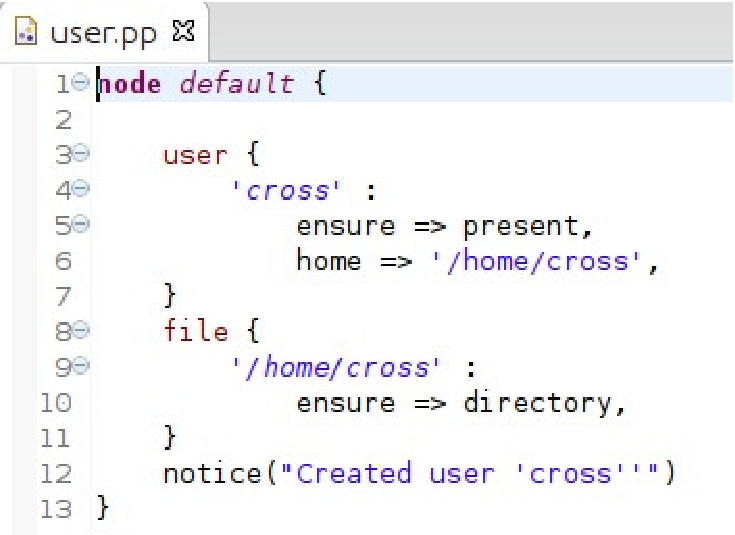
\includegraphics[width=0.7\textwidth]{images/user.pdf}
%  \end{center}
%  \caption{User mit Puppet anlegen}
%  \label{puppet-user}
%\end{figure}


%Der Manifest user.pp legen wir in einem Verzeichnis manifests ab\reffig{puppet-manifestdir}.

%\begin{figure}
%  \begin{center}
%    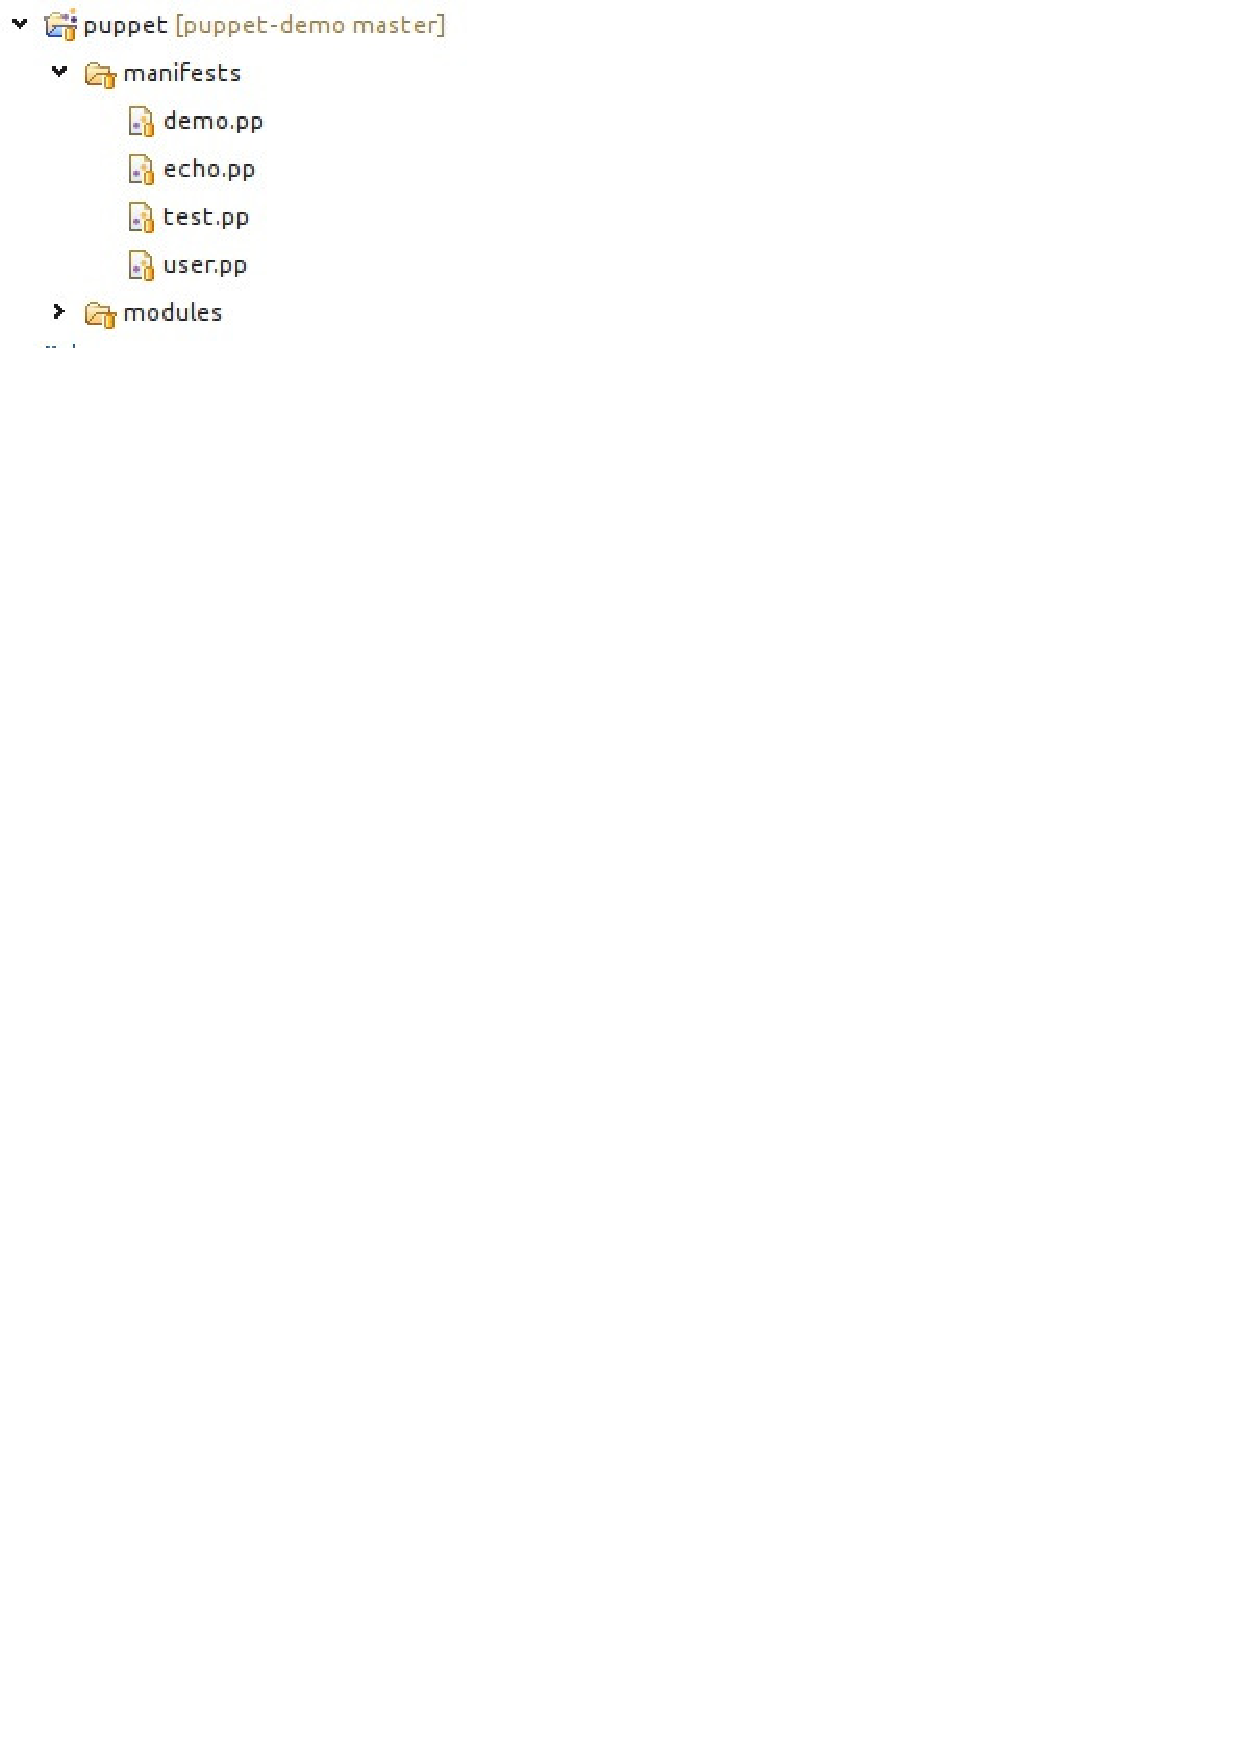
\includegraphics[width=0.7\textwidth]{images/manifestdir.pdf}
%  \end{center}
%  \caption{Puppet Manifest Verzeichnis}
%  \label{puppet-manifestdir}
%\end{figure}


\subsection{Testbox mit Vagrant}
Für die Entwicklung und Tests von Puppet Modulen und Manifeste empfielt sich eine virtuelle Machine. Puppet Labs stellt sollche für VMware und VirtualBox zur Verfügung unter \url{http://info.puppetlabs.com/download-learning-puppet-VM.html}. 

Eine andere Möglichkeit ist \cite{vagrant}. Vagrant ist eine Konfigurationstool für die Verwaltung von Virtuellen Maschinen mit VirtualBox. Es kann in weiterer Folge auch Puppet, Chef oder Shell Scripts benutzen kann um die virtuelle Maschine zu konfigurieren. Analog zu Virtualbox kann Vagrant via Paketmanager für Linux installiert werden oder von den entsprechenden Downloadseiten runtergeladen werden.Wir verwenden für diesen Artikel Vagrant. 

\begin{wrapfigure}{l}{5cm}
\vspace{-15pt}
\begin{boxedminipage}{5cm}
Eine Liste mit vorgefertigten Vagrant Boxen gibt es übrigens auf \url{http://www.vagrantbox.es/}
\end{boxedminipage}
\vspace{-15pt}
\end{wrapfigure}

Nachdem Vagrant und VirtualBox installiert worden sind, können wir eine Box zum Testen aufsetzen. In unserem Fall verwenden wir eine 64 Bit Version von Debian Squeeze. Diese wurde von uns für diesen Artikel neu erstellt und beinhaltet eine Minimalinstallation mit den für Vagrant üblichen Vorbereitungen: SSH Key Setup, VirtualBox Guest Additions, Puppet und Ruby. \url{http://vagrantup.com/v1/docs/base_boxes.html}

\begin{lstlisting}[language=sh,caption=Download der Vagrant Box, label=vagrant-add]
vagrant box add debian_squeeze_64 http://dl.dropbox.com/u/937870/VMs/squeeze64.box
\end{lstlisting}

\begin{wrapfigure}{r}{4.5cm}
\vspace{-20pt}
\begin{boxedminipage}{4.5cm}
 Die Vagrant Boxen werden unter Unix in installiert. \lstinline!$HOME/.vagrant.d/boxes!
Falls man dies ändern will kann man die Umgebungsvariable \lstinline$VAGRANT_HOME$ setzen:
\begin{lstlisting}[language=sh,label=vagrant-home,frame=none,numbers=none]
export VAGRANT_HOME=$HOME/vagrant_home
\end{lstlisting}
\end{boxedminipage}
\vspace{-20pt}
\end{wrapfigure}
 

Nachdem dem Download steht uns jetzt die  Vagrant Box \lstinline$debian_squeeze_64$ zur Verfügung. Nun können wir in ein beliebiges Verzeichnis wechseln und eine initiale Konfiguration basierend auf der Box anlegen\reflst{vagrant-init}.

\begin{lstlisting}[language=sh,caption=Vagrant initialisieren, label=vagrant-init]
vagrant init debian_squeeze_64
\end{lstlisting}

Diese initiale Konfiguration beinhaltet alles an was Vagrant zum Konfigurieren und Starten der Maschine braucht, es sind keine weiteren Einstellungen mehr nötig und wir können diese starten\reflst{vagrant-up}.

\begin{lstlisting}[language=sh,caption=Starten der Vagrant Maschine, label=vagrant-up]
vagrant up
\end{lstlisting}

Nachdem die virtuelle Machine gestartet worden ist, können wir mit ssh einsteigen\reflst{vagrant-ssh}. Unter Windows ist dieser Befehl derzeit nicht verfügbar und man muss deshalb mit Tools wie \cite{putty} darauf zugreifen.
\begin{lstlisting}[language=sh,caption=Mit ssh in der Vagrant Maschine einsteigen, label=vagrant-ssh]
vagrant ssh
\end{lstlisting}
 
Zum Aktivieren von Puppet müssen wir unseren Vagrantfile bearbeiten. Dieser liegt im Verzeichnis wo wir den Befehl \lstinline$vagrant init$ ausgeführt haben. Diese Datei beinhaltet bereits Einträge für Puppet, welche jedoch auskommentiert sind. Nach dem entfernen der Kommentarzeichen für die Sektion \lstinline$config.vm.provision :puppet$, tragen wir unter \lstinline$puppet.manifests_path$ und \lstinline$puppet.module_path$ ein wo unsere Manifeste und Module liegen. Als \lstinline$puppet.manifest_file$ tragen wir \lstinline$user.pp$ ein. Zum Testen von einer späteren Apache-Installation wird Port 6400 im Host auf Port 80 im Guest weitergeleitet:\lstinline$config.vm.forward_port 80, 6400$. Das ganze sollte dann in etwa wie in Listing \ref{vagrantprovisioning} aussehen.
  
\begin{lstlisting}[language=vagrant,caption=Puppet Provisioning in Vagrantfile konfigurieren, label=vagrantprovisioning]
  config.vm.forward_port 80, 6400  
  config.vm.provision :puppet do |puppet|
    puppet.manifests_path = "~/git/puppet-demo/puppet/manifests"
    puppet.module_path = "~/git/puppet-demo/puppet/modules"
    puppet.manifest_file  = "user.pp"
  end
\end{lstlisting} 

Bei dieser Änderung müssen wir den Box neu laden, da geteilte Verzeichnisse nur beim Starten des Hosts erkannt und automatisch gemounted werden. Zusätzlich dazu wird nun beim Starten das Provisioning durch Puppet mit den Anweisungen aus \lstinline$user.pp$ durchgeführt. Mit \lstinline$puppet ssh$ steigen wir und verifizieren dass der User 'puppetdemo' mit Home-Verzeichnis /home/puppetdemo vorhanden ist\reflst{vagrant-reload}.

\begin{lstlisting}[language=sh,caption=Vagrant Box neu laden, label=vagrant-reload]
vagrant reload
notice: /Stage[main]//Node[default]/User[puppetdemo]/ensure: created
notice: /Stage[main]//Node[default]/File[/home/puppetdemo]/ensure: created
notice: Finished catalog run in 0.35 seconds

$ vagrant ssh
Welcome to your Vagrant-built virtual machine.

$ sudo su - puppetdemo
puppetdemo@precise32:~$ pwd
/home/puppetdemo
\end{lstlisting}

Mit \lstinline$vagrant provisioning$ kann das Puppet Manifest erneut ausgeführt werden. Ohne Änderungen im Manifest oder in der virtuellen Maschine passiert nichts. Würde der Benutzer \lstinline$puppetdemo$ zum Beispiel entfernt, wird er wieder beim nächsten Provisionvorgang wieder angelegt.
Will man das Puppet Manifest in der virtuellen Maschine ausführen, ist der \lstinline$puppet.manifests_path$ als \lstinline$/tmp/vagrant-puppet/manifest$ gemounted\reflst{vagrant-apply}.

\begin{lstlisting}[language=sh,caption=Puppet apply im Box, label=vagrant-apply]
$ sudo puppet apply /tmp/vagrant-puppet/manifests/user.pp
No LSB modules are available.
notice: Finished catalog run in 0.04 seconds
$ sudo deluser puppetdemo
Removing user `puppetdemo' ...
Warning: group `puppetdemo' has no more members.
Done.
$ sudo puppet apply /tmp/vagrant-puppet/manifests/user.pp
No LSB modules are available.
notice: /Stage[main]//Node[default]/User[puppetdemo]/ensure: created
notice: Finished catalog run in 0.39 seconds
\end{lstlisting}

Vagrant kann wie VirtualBox die Maschine stilllegen mit \lstinline$vagrant suspend$ bzw mit \lstinline$vagrant resume$ wieder fortsetzen. Zum Starten und Stoppen kann man \lstinline$vagrant up$ bzw mit \lstinline$vagrant halt$ verwenden.  Sollte man die Box nicht mehr benötigen kann Sie mit \lstinline$vagrant destroy$ unwiderruflich löschen. Das Vagrantfile bleibt jedoch erhalten, somit damit kann man wieder bei Null anfangen und mit \lstinline$vagrant up$ die Box inklusive Provisioning mit Puppet wieder aufsetzen.

\section{Apache Webserver und eine Applikation mit HTML und JavaScript mit Puppet installieren}
Nachdem wir die Grundlagen von Puppet und Vagrant jetzt kurz kennengelernt haben, installieren wir einen Apache Webserver. Da es wahrscheinlich ist, dass Apache für andere Applikationen auch genutzt wird, wird der Puppet Code dafür in einem Module abgelegt. Module sind wiederverwendbare Einheiten vom Code und Daten. Die Struktur eines Modules ist auf \url{http://docs.puppetlabs.com/learning/modules1.html} beschrieben\reflst{module_structure} bzw. im Puppet Module Cheat Sheet \url{docs.puppetlabs.com/module_cheat_sheet.pdf} auch noch einmal zusammengefasst.

\begin{lstlisting}[language=tree,caption=Puppet Module Struktur, label=module_structure]
my_module
|-- files
|   `-- my_file.txt
|-- manifests
|   `-- init.pp
`-- templates
    `-- my_template.erb
\end{lstlisting}


Auf die gleiche Ebene wie das manifests-Verzeichnis legen wir das Verzeichnis \lstinline$modules$ an. Darunter die Datei und darunter liegenden Verzeichnisse \lstinline$apache/manifests/init.pp$\reflst{apache-module}.
%use to generate this tree --noreport -n puppet
\begin{lstlisting}[language=tree,caption=Verzeichnisstruktur für den apache-Module, label=apache-module]
puppet
|-- manifests
|   `-- user.pp
`-- modules
    `-- apache
        `-- manifests
            `-- init.pp
\end{lstlisting}

\lstinline$modules/apache/manifests/init.pp$ ist recht kompakt und zeigt auf einen Blick einen der großen Vorteile von Puppet. Die Ressourcen \lstinline$package$ und \lstinline$service$ verstecken die Komplexität und die plattformspezifische Vorgänge für Installation von Paketen und das Starten der Dienste\reflst{apache-init.pp}.
\begin{lstlisting}[language=puppet,caption=Inhalt von modules/apache/manifests/init.pp, label=apache-init.pp]
class apache {
        package {
                'apache2' :
                        ensure => present,
        }
        service {
                'apache2' :
                        ensure => running,
                        require => Package["apache2"]
        }
}
\end{lstlisting}

Um ein Module in einem Manifest verwenden zu können, reicht es lediglich \lstinline$include apache$\reflst{setupapache.pp} zu schreiben.
\begin{lstlisting}[language=puppet,caption=Inhalt von manifests/setupapache.pp, label=setupapache.pp]
include apache
\end{lstlisting}

In Vagrantfile ändern wir jetzt die Zeile \lstinline$puppet.manifest_file  = "user.pp"$ auf \lstinline$puppet.manifest_file  = "setupapache.pp"$ und geben auf der Kommandozeile \lstinline$vagrant provision$ ein\reflst{provisioning_apache}.

\begin{lstlisting}[language=sh,caption=vagrant provisioning für Apache, label=provisioning_apache]
$ vagrant provision
[default] Running provisioner: Vagrant::Provisioners::Puppet...
[default] Running Puppet with /tmp/vagrant-puppet/manifests/setupapache.pp...
notice: /Stage[main]/Apache/Package[apache2]/ensure: ensure changed 'purged' to 'present'
notice: Finished catalog run in 97.25 seconds
\end{lstlisting}

Wenn wir auf unseren Browser die lokale Adresse über, den weitergeleiteten, Port 6400 aufrufen, können wir feststellen dass der Apache Webserver läuft\reffig{apache}.
\begin{figure}
  \begin{center}
    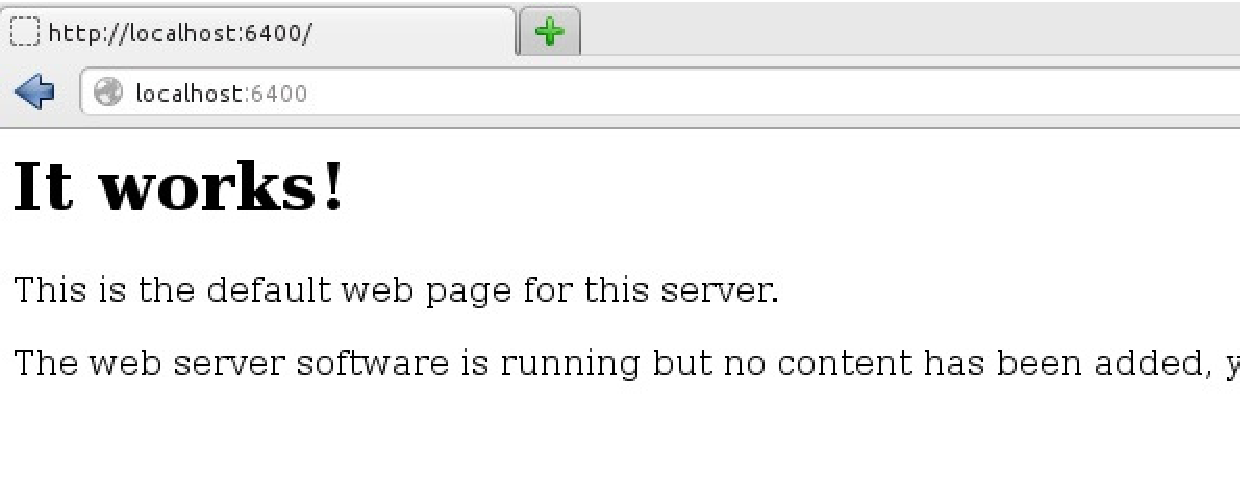
\includegraphics[width=0.4\textwidth]{images/apache.pdf}
  \end{center}
  \caption{Apache aufrufen}
  \label{apache}
\end{figure}

Als nächstes lassen wir Puppet die Dateien für die Applikation in das Verzeichnis für \lstinline$DocumentRoot/var/www/$ kopieren. Folgender Eintrag in Vagrantfile stellt das Host-Verzeichnis \lstinline$~/git/puppet-demo/puppet-demoapp/src/main/webapp$ als Guest-Verzeichnis \lstinline$/demoapp$ zur Verfügung\reflst{vagrantsharedfolder}. Das Guest-Verzeichnis dient als Quelle für die Kopie.
\begin{lstlisting}[language=vagrant,caption=Shared folders in Vagrantfile konfigurieren, label=vagrantsharedfolder]
config.vm.share_folder "demoapp", "/demoapp", "~/git/puppet-demo/puppet-demoapp/src/main/webapp"
\end{lstlisting}

Mit dem Manifest \lstinline$manifests/demoapp.pp$ für die Installation der Applikation\reflst{puppetdemoapp}, definieren wir das Puppet die Dateien vom zuvor spezifizierten Verzeichnis \lstinline$/demoapp$ nach \lstinline$/var/www/$ kopieren sollen.
\begin{lstlisting}[language=puppet,caption=Puppet Manifest für die Applikation, label=puppetdemoapp]
include apache

file { '/var/www/demoapp' :
  ensure => directory,
  source  => '/demoapp',
  require => Package['apache2'],
  recurse => true,
}
\end{lstlisting}

Durch die Änderung der geteilten Verzeichnisse im Vagrantfile ist es notwendig die Vagrant Box neu zu starten um die Änderung aktiv werden zu lassen:\lstinline$vagrant reload$\reflst{reloaddemoapp}.
\begin{lstlisting}[language=sh,caption=Puppet reload mit Provisioning der Applikation, label=reloaddemoapp]
$ vagrant reload
[default] Attempting graceful shutdown of VM...
[default] Clearing any previously set forwarded ports...
[default] Forwarding ports...
[default] -- 22 => 2222 (adapter 1)
[default] -- 80 => 6400 (adapter 1)
[default] Creating shared folders metadata...
[default] Clearing any previously set network interfaces...
[default] Booting VM...
[default] Waiting for VM to boot. This can take a few minutes.
[default] VM booted and ready for use!
[default] Mounting shared folders...
[default] -- demoapp: /demoapp
[default] -- v-root: /vagrant
[default] -- v-pp-m0: /tmp/vagrant-puppet/modules-0
[default] -- manifests: /tmp/vagrant-puppet/manifests
[default] Running provisioner: Vagrant::Provisioners::Puppet...
[default] Running Puppet with /tmp/vagrant-puppet/manifests/demoapp.pp...
notice: /Stage[main]//File[/var/www/demoapp]/ensure: created
...
notice: /File[/var/www/demoapp/index.html]/ensure: defined content as '{md5}90a8d419b9c7b43b09ba73abebaf8f4c'
...
notice: Finished catalog run in 1.34 seconds
\end{lstlisting}

Nach Abschluss des Neustarts erfolgt auch automatisch wieder der Provision Vorgang durch Puppet und wir können unsere neue Webapplikation über den Browser aufrufen\reffig{demoapp}.
\begin{figure}
  \begin{center}
    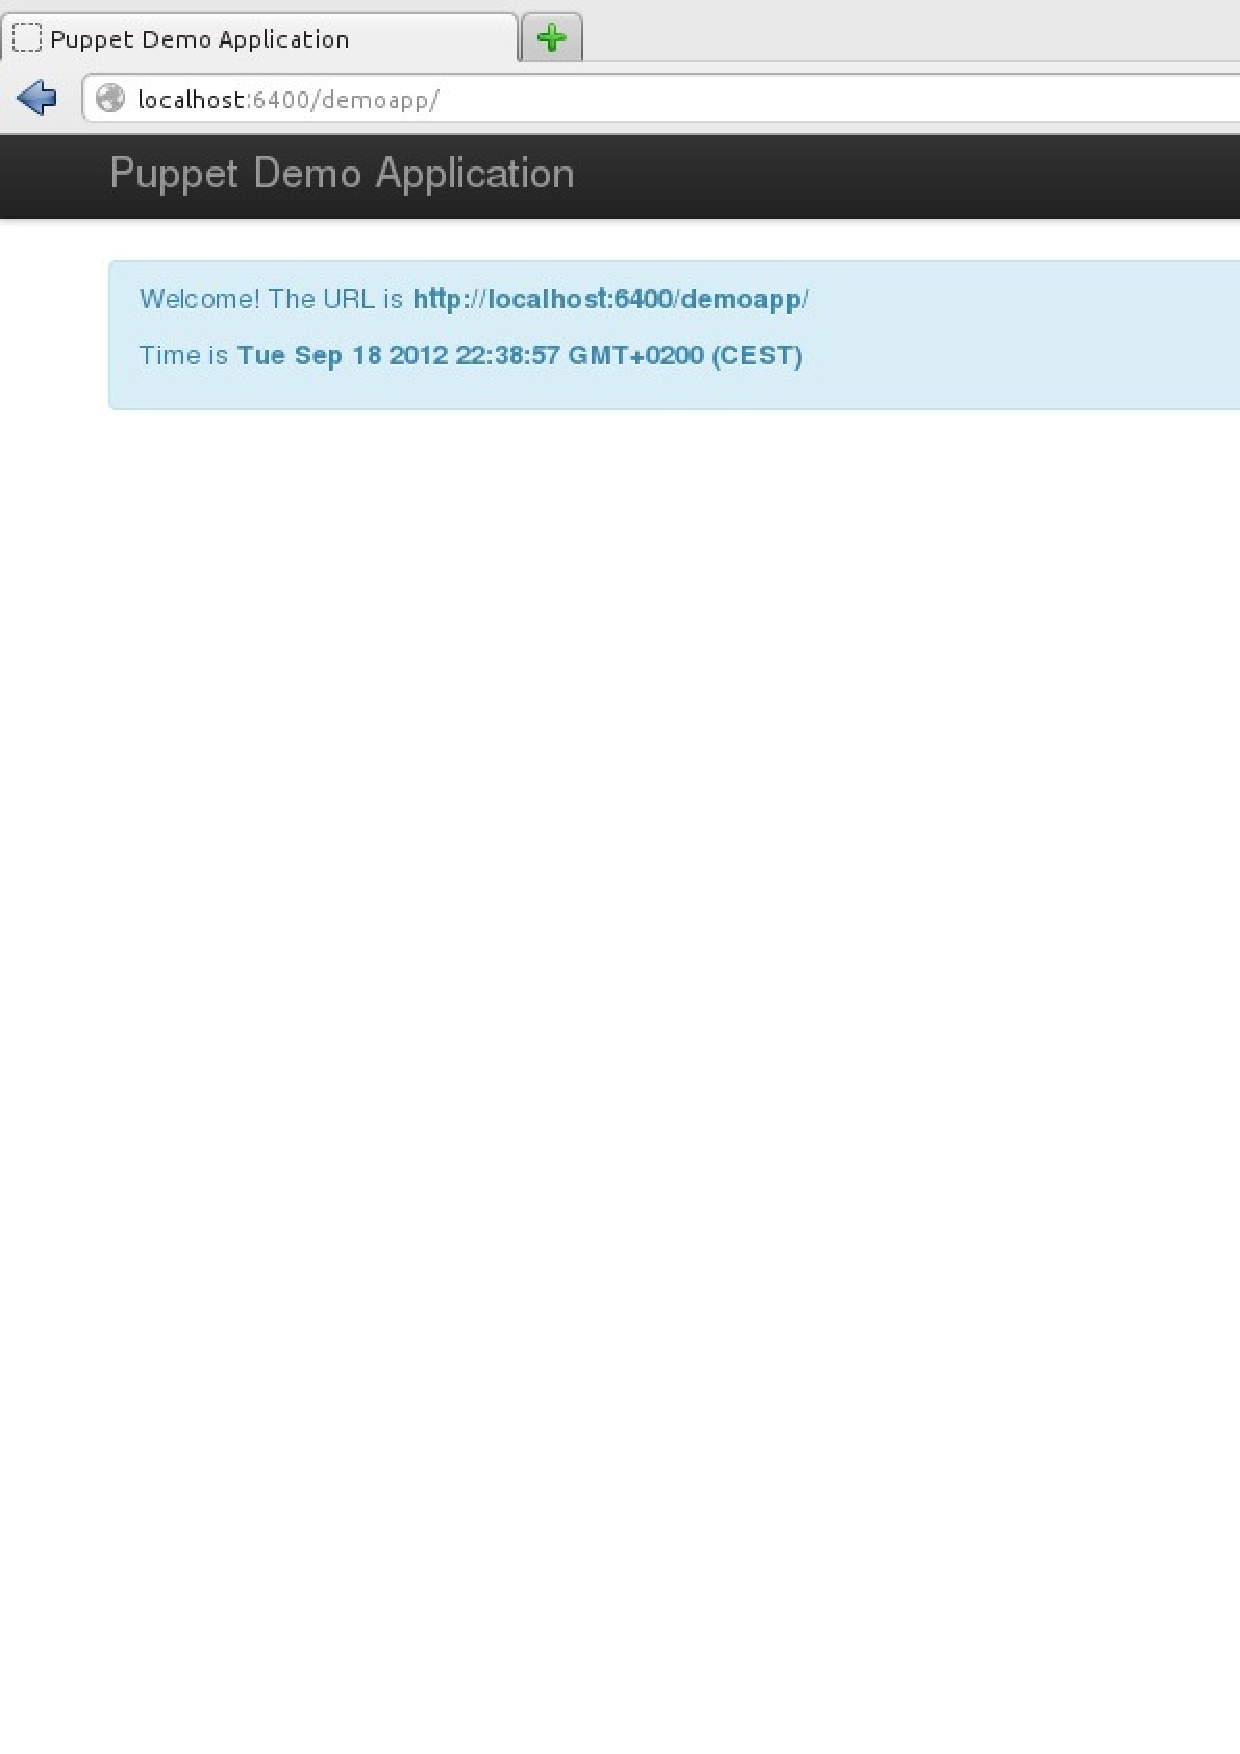
\includegraphics[width=0.4\textwidth]{images/demoapp.pdf}
  \end{center}
  \caption{Die Applikation im Browser}
  \label{demoapp}
\end{figure}

Eine Änderung in der Datei \lstinline$index.html$ wird bei Puppet im Provisioning-Vorgang (\lstinline$vagrant provision$) erkannt und Puppet aktualisiert die Datei auch in \lstinline$/var/www/$\reflst{provisionapp}.
\begin{lstlisting}[language=sh,caption=Puppet Provisioning nach Änderung von index.html, label=provisionapp]
$ vagrant provision
[default] Running provisioner: Vagrant::Provisioners::Puppet...
[default] Running Puppet with /tmp/vagrant-puppet/manifests/demoapp.pp...

notice: /File[/var/www/demoapp/index.html]/content: content changed '{md5}90a8d419b9c7b43b09ba73abebaf8f4c' to '{md5}0a4ee5bb63c3e5c29cc54cf36a4be23c'

notice: Finished catalog run in 0.71 seconds
\end{lstlisting}


\section*{Autoren}

\newcommand{\authorboxheight}{5cm}
\begin{minipage}[t][\authorboxheight]{0.45\textwidth}
\textbf{Anders Malmborg}
\vskip0.3cm
\begin{wrapfigure}{l}{0.3\textwidth}
\vspace{-20pt}

\includegraphics[width=0.3\textwidth]{images/anders.jpg}
\vspace{-20pt}
\end{wrapfigure}
hat jahrezehntelange Erfahrung in Applikations und Produktentwicklung im C++ und JavaEE  und arbeitet als IT Freelancer im automotive Bereich. 
\end{minipage}
\hspace{0.1\textwidth}
\begin{minipage}[t][\authorboxheight]{0.45\textwidth}
\textbf{Michael Haslgrübler}
\vskip0.3cm
\begin{wrapfigure}{l}{0.3\textwidth}
\vspace{-20pt}

\includegraphics[width=0.3\textwidth]{images/michael.jpg}
\vspace{-20pt}
\end{wrapfigure}
hat mehrjährige Erfahrung in JavaEE Entwicklungsumfeld in der Automotive und Immobilienbranche. Er administriert seit Jahren einen Linux-Root-Server für diverse Kunden.
\end{minipage}

\bibliographystyle{apalike2}
\bibliography{document}

\end{document}
